\chapter{Implémentation Technique}

\section{Infrastructure et Ingestion}

L'infrastructure de base repose sur des conteneurs Docker pour Zookeeper, Kafka et Flink. Le composant d'ingestion est un simulateur développé en Python (\texttt{simulateur.py}) qui génère des événements de navigation (vues, ajouts au panier, achats, abandons) et les envoie dans le topic Kafka \texttt{clics\_ecommerce}.

\begin{borderedfigure}
    \centering
    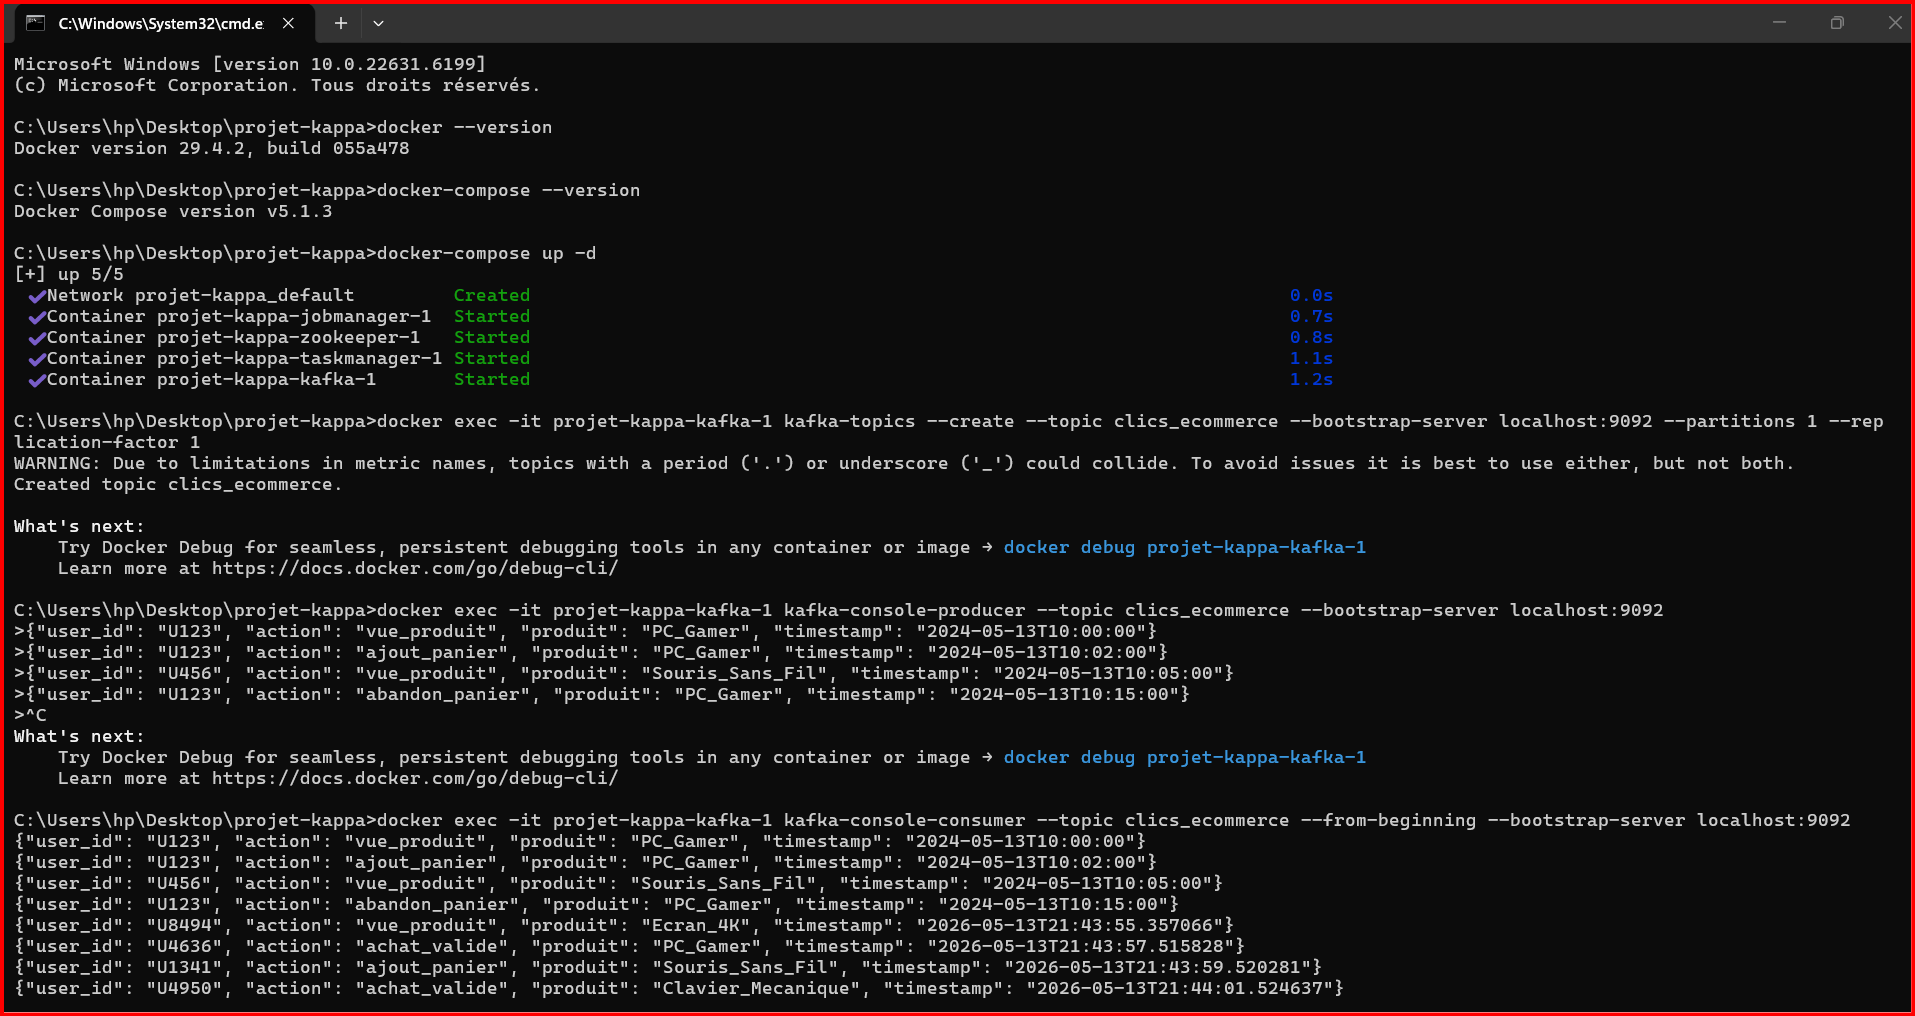
\includegraphics[width=0.8\textwidth]{../screenshots/2.png}
    \captionof{figure}{Démarrage des conteneurs Docker et création des topics}
\end{borderedfigure}

\section{Topologies de Traitement}

Conformément à l'architecture Kappa, les données traversent plusieurs topologies de traitement événementiel :

\subsection{Topologie de Filtrage}
Elle lit le flux brut et élimine les événements générés par des robots.
\begin{borderedfigure}
    \centering
    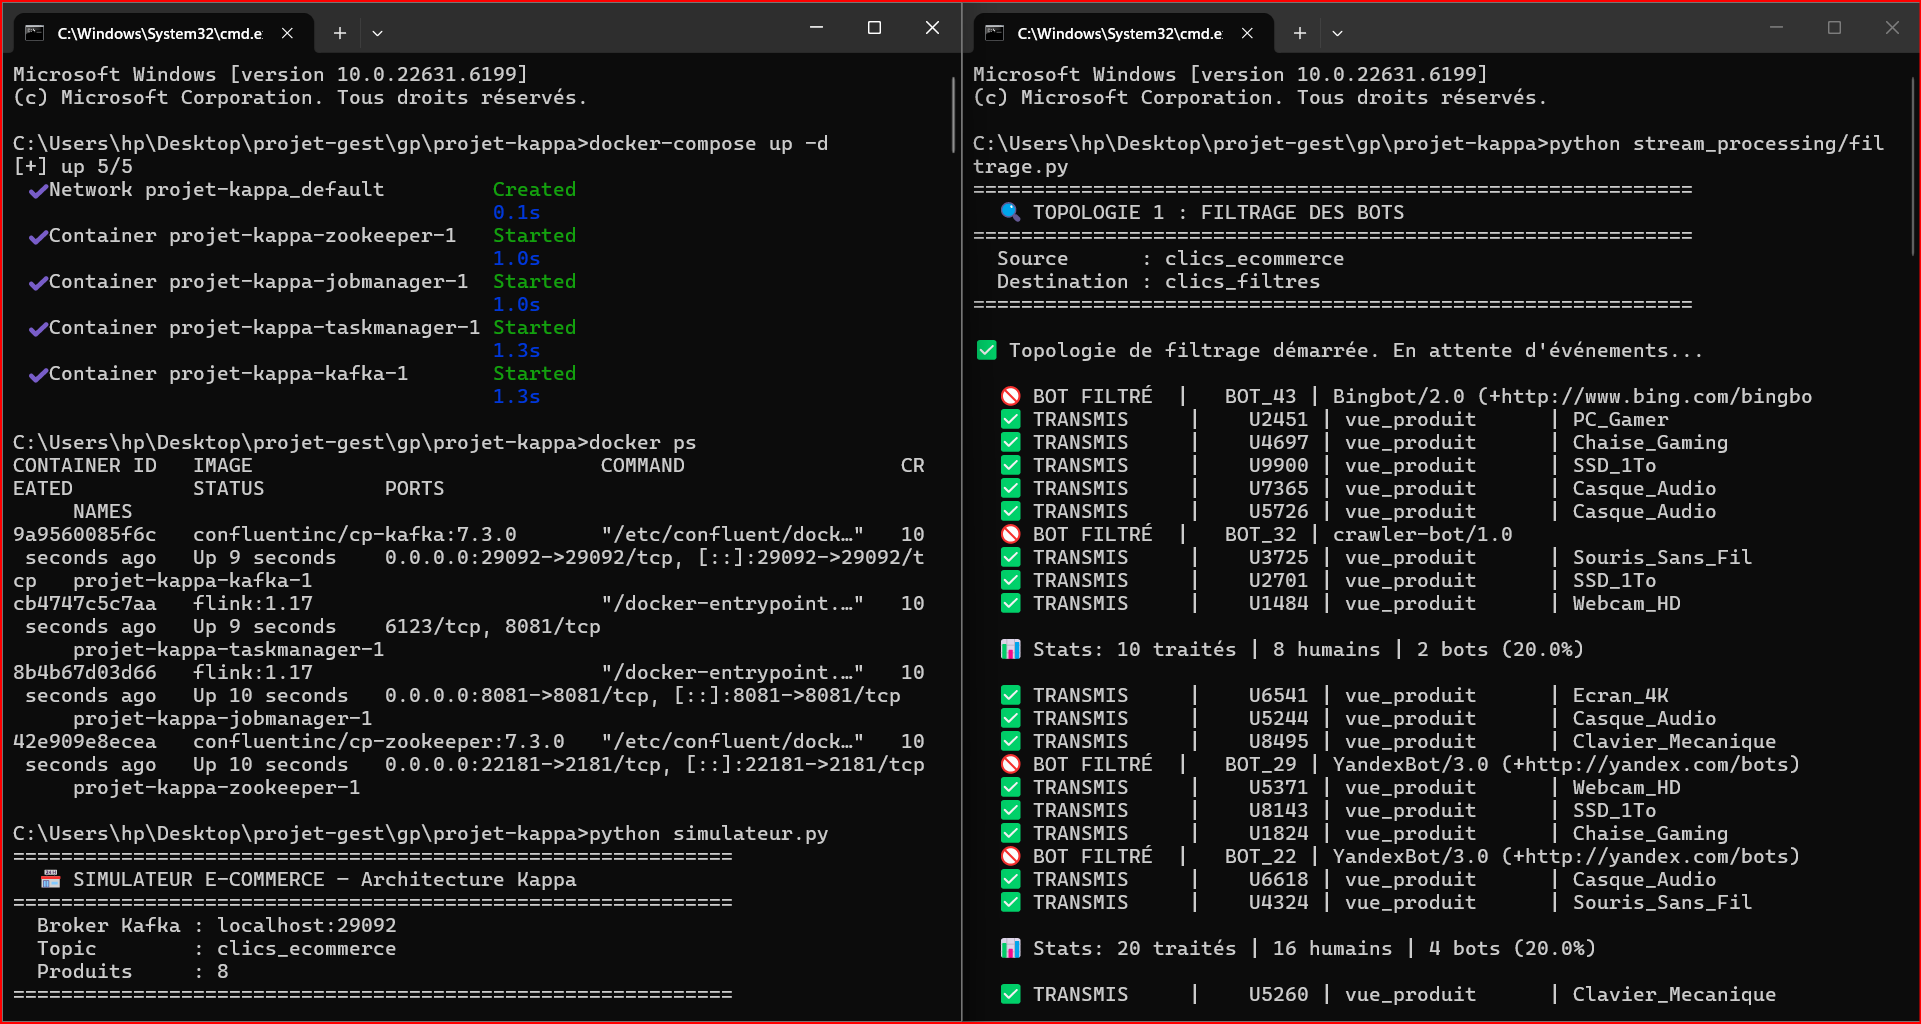
\includegraphics[width=\textwidth]{../screenshots/filtrage_bots.png}
    \captionof{figure}{Topologie de filtrage séparant les utilisateurs légitimes des robots}
\end{borderedfigure}

\subsection{Topologie d'Agrégation}
Elle calcule la somme des paniers et le nombre de vues en temps réel par des fenêtres glissantes de 30 secondes.
\begin{borderedfigure}
    \centering
    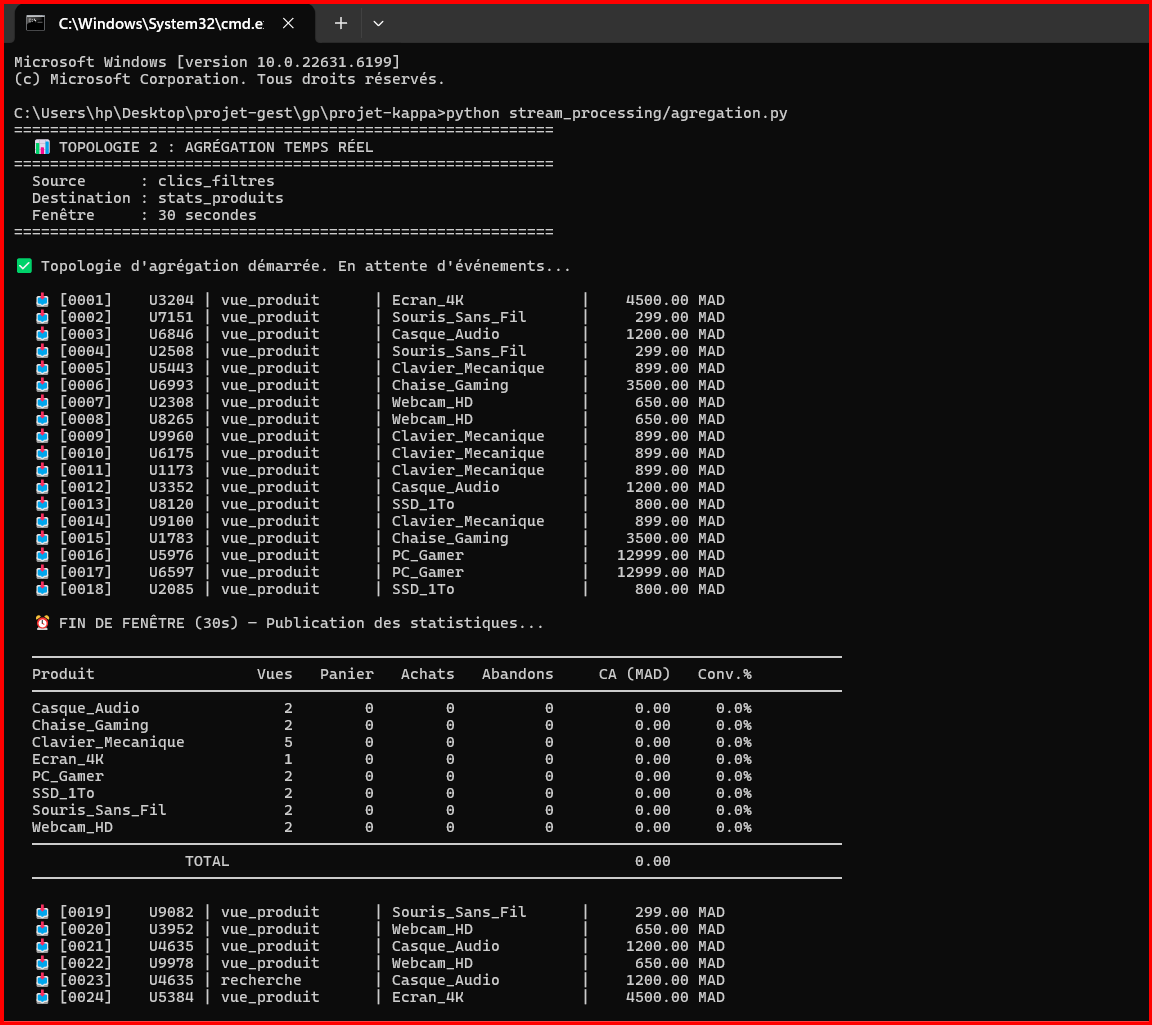
\includegraphics[width=\textwidth]{../screenshots/agregation_stats.png}
    \captionof{figure}{Agrégation en temps réel des statistiques par produit}
\end{borderedfigure}

\subsection{Topologie de Détection d'Abandon}
Elle maintient un état en mémoire pour identifier les abandons de panier et déclencher une alerte marketing immédiate après 60 secondes d'inactivité.
\begin{borderedfigure}
    \centering
    \includegraphics[width=\textwidth]{../screenshots/alerte_abandon.png}
    \captionof{figure}{Déclenchement d'une alerte marketing d'abandon de panier}
\end{borderedfigure}

\section{Rétention et Replay}

La particularité de Kappa est la gestion de la rétention des événements. Nous avons configuré une \textbf{rétention de 7 jours} sur le topic principal. En cas de changement de logique ou d'audit, il est possible de rejouer tout l'historique (\texttt{--from-beginning}) pour recalculer les statistiques. C'est le test de cohérence.

\begin{borderedfigure}
    \centering
    \includegraphics[width=\textwidth]{../screenshots/validation_replay.png}
    \captionof{figure}{Test de Replay validant la parfaite cohérence avec le traitement temps réel}
\end{borderedfigure}
